%iffalse
\let\negmedspace\undefined
\let\negthickspace\undefined
\documentclass[journal,12pt,onecolumn]{IEEEtran}
\usepackage{cite}
\usepackage{amsmath,amssymb,amsfonts,amsthm}
\usepackage{algorithmic}
\usepackage{graphicx}
\usepackage{textcomp}
\usepackage{xcolor}
\usepackage{txfonts}
\usepackage{listings}
\usepackage{enumitem}
\usepackage{mathtools}
\usepackage{gensymb}
\usepackage{comment}
\usepackage[breaklinks=true]{hyperref}
\usepackage{tkz-euclide} 
\usepackage{listings}
\usepackage{booktabs}
\usepackage{pgfplots}
\usepackage{gvv}                                        
\usepackage[latin1]{inputenc}     
\usepackage{xparse}
\usepackage{color}                                            
\usepackage{array}                                            
\usepackage{longtable}                                       
\usepackage{calc}                                             
\usepackage{multirow}
\usepackage{multicol}
\usepackage{hhline}                                           
\usepackage{ifthen}                                           
\usepackage{lscape}
\usepackage{tabularx}
\usepackage{array}
\usetikzlibrary{patterns}
\usepackage{float}
\newtheorem{theorem}{Theorem}[section]
\newtheorem{problem}{Problem}
\newtheorem{proposition}{Proposition}[section]
\newtheorem{lemma}{Lemma}[section]
\newtheorem{corollary}[theorem]{Corollary}
\newtheorem{example}{Example}[section]
\newtheorem{definition}[problem]{Definition}
\newcommand{\BEQA}{\begin{eqnarray}}
\newcommand{\EEQA}{\end{eqnarray}}
\newcommand{\define}{\stackrel{\triangle}{=}}
\theoremstyle{remark}
\newtheorem{rem}{Remark}
% Marks the beginning of the document
\pgfplotsset{compat=1.18}
\begin{document}



\bibliographystyle{IEEEtran}
\vspace{3cm}


\title{2021-XE-'1-13'}
\author{EE24BTECH11023}
%\maketitle
%\newpage
%\bigskip
\maketitle

\section*{General Aptitude (GA)}

\subsection*{Q.1 - Q.5 Multiple Choice Questions (MCQs),carry \textbf{ONE} mark each. (For each wrong answer: $-\frac{1}{3}$).}


{\let\newpage\relax\maketitle}

\renewcommand{\thefigure}{\theenumi}
\renewcommand{\thetable}{\theenumi}
\setlength{\intextsep}{10pt} % Space between text and floats


\numberwithin{equation}{enumi}
\numberwithin{figure}{enumi}
\renewcommand{\thetable}{\theenumi}


\begin{enumerate}
    \item Gauri said that she can play the keyboard {\underline{\hspace{2cm}}} her sister.
    \begin{enumerate}
        \item as well as
        \item as better as
        \item as nicest as
        \item as worse as
    \end{enumerate}

    \item A transparent square sheet shown below is folded along the dotted line. The folded sheet will look like {\underline{\hspace{2cm}}}.
     \begin{figure}[H]
        \centering
        
    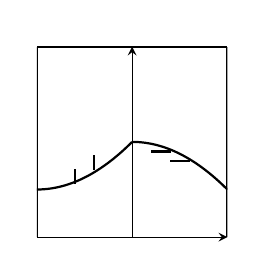
\begin{tikzpicture}
        \begin{axis}[
            axis lines = middle,
            xlabel = $ $,
            ylabel = $ $,
            xmin = -0.5, xmax = 0.5,
            ymin = 0, ymax = 1,
            xtick = {0},
            ytick = {0},
            x label style={at={(axis description cs:1,0)},anchor=west},
            y label style={at={(axis description cs:0,1)},anchor=south},
            extra tick style={grid=major},
            width=4cm, height=4cm,
            samples=100,
            domain=-0.5:0.5,
        ]
                \addplot[domain=-0.5:0, samples=100, thick] {0.25+(x+0.5)^2};
\draw [thick](-0.5,0) -- (-0.5,1);
\draw [thick](0.5,0) -- (0.5,1);
\draw [thick](0.5,1) -- (-0.5,1);
                \addplot[domain=0.1:0.2, samples=100, thick] {0.45};
                \addplot[domain=0.2:0.3, samples=100, thick] {0.40};
             \draw [thick](-0.2,0.35) -- (-0.2,0.43);
                          \draw [thick](-0.3,0.28) -- (-0.3,0.36);





        \addplot[domain=0:0.5, samples=100, thick] {0.5-x^2};



        \end{axis}
    \end{tikzpicture}
    
  % Use the correct path to your Q4.tex file
    \end{figure}
       
   
    \begin{enumerate}
        \item  \begin{figure}[H]
        
        
    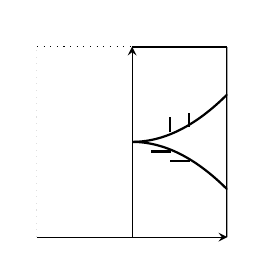
\begin{tikzpicture}
        \begin{axis}[
            axis lines = middle,
            xlabel = $ $,
            ylabel = $ $,
            xmin = -0.5, xmax = 0.5,
            ymin = 0, ymax = 1,
            xtick = {0},
            ytick = {0},
            x label style={at={(axis description cs:1,0)},anchor=west},
            y label style={at={(axis description cs:0,1)},anchor=south},
            extra tick style={grid=major},
            width=4cm, height=4cm,
            samples=100,
            domain=-0.5:0.5,
        ]
\draw [thick](0.5,0) -- (0.5,1);
\draw [thick](0.5,1) -- (0,1);
                \addplot[domain=0.1:0.2, samples=100, thick] {0.45};
                \addplot[domain=0.2:0.3, samples=100, thick] {0.40};
           \draw [dotted](-0.5,0) -- (-0.5,1);
\draw [dotted](-0.5,1) -- (0,1);
\draw [dotted](0,0) -- (-0.5,0);
        \draw [thick](0.2,0.55) -- (0.2,0.63);
                          \draw [thick](0.3,0.58) -- (0.3,0.65);





        \addplot[domain=0:0.5, samples=100, thick] {0.5-x^2};
                \addplot[domain=0:0.5, samples=100, thick] {0.5+x^2};




        \end{axis}
    \end{tikzpicture}
    
  % Use the correct path to your Q4.tex file
    \end{figure}
       
        \item  \begin{figure}[H]
        
        
    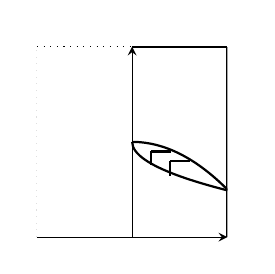
\begin{tikzpicture}
        \begin{axis}[
            axis lines = middle,
            xlabel = $ $,
            ylabel = $ $,
            xmin = -0.5, xmax = 0.5,
            ymin = 0, ymax = 1,
            xtick = {0},
            ytick = {0},
            x label style={at={(axis description cs:1,0)},anchor=west},
            y label style={at={(axis description cs:0,1)},anchor=south},
            extra tick style={grid=major},
            width=4cm, height=4cm,
            samples=100,
            domain=-0.5:0.5,
        ]
\draw [thick](0.5,0) -- (0.5,1);
\draw [thick](0.5,1) -- (0,1);
                \addplot[domain=0.1:0.2, samples=100, thick] {0.45};
                \addplot[domain=0.2:0.3, samples=100, thick] {0.40};
           \draw [dotted](-0.5,0) -- (-0.5,1);
\draw [dotted](-0.5,1) -- (0,1);
\draw [dotted](0,0) -- (-0.5,0);
        \draw [thick](0.1,0.45) -- (0.1,0.38);
                          \draw [thick](0.2,0.40) -- (0.2,0.32);





        \addplot[domain=0:0.5, samples=100, thick] {0.5-x^2};
                \addplot[domain=0:0.5, samples=100, thick] {(-(0.36*x^(0.5))+0.5};




        \end{axis}
    \end{tikzpicture}
    
  % Use the correct path to your Q4.tex file
    \end{figure}
       
        \item  \begin{figure}[H]
        
    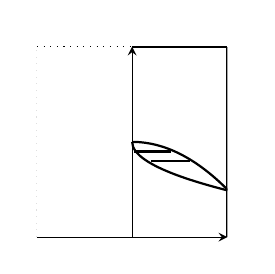
\begin{tikzpicture}
        \begin{axis}[
            axis lines = middle,
            xlabel = $ $,
            ylabel = $ $,
            xmin = -0.5, xmax = 0.5,
            ymin = 0, ymax = 1,
            xtick = {0},
            ytick = {0},
            x label style={at={(axis description cs:1,0)},anchor=west},
            y label style={at={(axis description cs:0,1)},anchor=south},
            extra tick style={grid=major},
            width=4cm, height=4cm,
            samples=100,
            domain=-0.5:0.5,
        ]
\draw [thick](0.5,0) -- (0.5,1);
\draw [thick](0.5,1) -- (0,1);
                \addplot[domain=0.01:0.2, samples=100, thick] {0.45};
                \addplot[domain=0.1:0.3, samples=100, thick] {0.40};
           \draw [dotted](-0.5,0) -- (-0.5,1);
\draw [dotted](-0.5,1) -- (0,1);
\draw [dotted](0,0) -- (-0.5,0);
      





        \addplot[domain=0:0.5, samples=100, thick] {0.5-x^2};
                \addplot[domain=0:0.5, samples=100, thick] {(-(0.36*x^(0.5))+0.5};




        \end{axis}
    \end{tikzpicture}
    
  % Use the correct path to your Q4.tex file
    \end{figure}
       
        \item  \begin{figure}[H]
        
    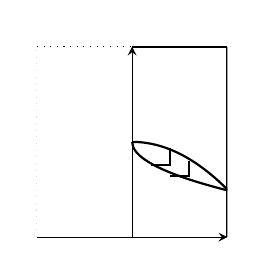
\begin{tikzpicture}
        \begin{axis}[
            axis lines = middle,
            xlabel = $ $,
            ylabel = $ $,
            xmin = -0.5, xmax = 0.5,
            ymin = 0, ymax = 1,
            xtick = {0},
            ytick = {0},
            x label style={at={(axis description cs:1,0)},anchor=west},
            y label style={at={(axis description cs:0,1)},anchor=south},
            extra tick style={grid=major},
            width=4cm, height=4cm,
            samples=100,
            domain=-0.5:0.5,
        ]
\draw [thick](0.5,0) -- (0.5,1);
\draw [thick](0.5,1) -- (0,1);
                \addplot[domain=0.1:0.2, samples=100, thick] {0.38};
                \addplot[domain=0.2:0.3, samples=100, thick] {0.32};
           \draw [dotted](-0.5,0) -- (-0.5,1);
\draw [dotted](-0.5,1) -- (0,1);
\draw [dotted](0,0) -- (-0.5,0);
        \draw [thick](0.2,0.47) -- (0.2,0.38);
                          \draw [thick](0.3,0.40) -- (0.3,0.32);





        \addplot[domain=0:0.5, samples=100, thick] {0.5-x^2};
                \addplot[domain=0:0.5, samples=100, thick] {(-(0.36*x^(0.5))+0.5};




        \end{axis}
    \end{tikzpicture}
    
  % Use the correct path to your Q4.tex file
    \end{figure}
       
    \end{enumerate}
    
    \item If $\theta$ is the angle, in degrees, between the longest diagonal of the cube and any one of the edges of the cube, then $\cos \theta =$
    \begin{enumerate}
        \item $\frac{1}{2}$
        \item $\frac{1}{\sqrt{3}}$
        \item $\frac{1}{\sqrt{2}}$
        \item $\frac{\sqrt{3}}{2}$
    \end{enumerate}

    \item If $(x- \frac{1}{2})^2-(x- \frac{3}{2})^2=x+2$, then the value of $x$ is:
    \begin{enumerate}
        \item 2
        \item 4
        \item 6
        \item 8
    \end{enumerate}
    
    \item Pen : Write :: Knife : {\underline{\hspace{2cm}}}\\
    Which one of the following options maintains a similar logical relation in the above?
    \begin{enumerate}
        \item Vegetables
        \item Sharp
        \item Cut
        \item Blunt
    \end{enumerate}
\end{enumerate}

\subsection*{Q.6 - Q.10 Multiple Choice Questions (MCQs),carry \textbf{TWO} marks each. (For each wrong answer: $-\frac{2}{3}$).
}

\begin{enumerate}
    \setcounter{enumi}{5}
    \item Listening to music during exercise improves exercise performance and reduces discomfort. Scientists researched whether listening to music while studying can help students learn better, and the results were inconclusive. Students who needed external stimulation for studying fared worse while students who did not need any external stimulation benefited from music.
    
    Which one of the following statements is the \textbf{CORRECT} inference of the above passage?
    \begin{enumerate}
        \item Listening to music has no effect on learning and a positive effect on physical exercise.
        \item Listening to music has a clear positive effect both on physical exercise and on learning.
        \item Listening to music has a clear positive effect on physical exercise. Music has a positive effect on learning only in some students.
        \item Listening to music has a clear positive effect on learning in all students. Music has a positive effect only in some students who exercise.
    \end{enumerate}

    \item A jigsaw puzzle has two pieces. One of the pieces is shown below. Which one of the given options for the missing piece when assembled will form a rectangle? The piece can be moved, rotated or flipped to assemble with the above piece.
     \begin{figure}[H]
        \centering
        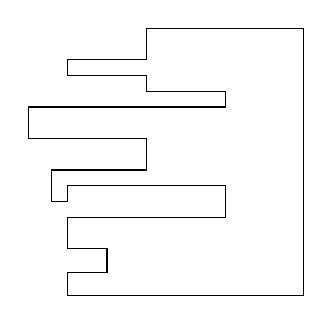
\begin{tikzpicture}
        \draw (0,0.6) -- (3,0.6) -- (3,4) -- (1,4) -- (1,3.6) -- (0,3.6) -- (0,3.4) -- (1,3.4) --  (1,3.2) -- (2,3.2) -- (2,3) -- (-0.5,3)--(-0.5,2.6) -- (1,2.6) -- (1,2.2) -- (-0.2,2.2) -- (-0.2,1.8) -- (0,1.8) -- (0,2) --  (2,2) -- (2,1.6) -- (0,1.6) -- (0,1.2)--(0.5,1.2)--(0.5,0.9)--(0,0.9) -- cycle;
    \end{tikzpicture}

  % Use the correct path to your Q4.tex file
    \end{figure}
       
   
    \begin{enumerate}
        \item  \begin{figure}[H]
        \centering
         \begin{tikzpicture}
            \draw (0.3,0) -- (4,0) -- (4,2) -- (3.5,2) --(3.5,1.3)--(3.2,1.3)--(3.2,2) --(2.9,2)--(2.9,3)--(2.7,3)--(2.7,0.9)--(2.4,0.9)--(2.4,2.5)--(2,2.5)--(2,1.6)--(1.6,1.6)--(1.6,1.8)--(1.8,1.8)--(1.8,3.4)--(1.4,3.4)--(1.4,2)--(0.9,2)--(0.9,2.6)--(0.6,2.6)--(0.6,2)--(0.3,2)--(0.3,0) -- cycle;
        \end{tikzpicture}
  % Use the correct path to your Q4.tex file
    \end{figure}
       
        \item  \begin{figure}[H]
        \centering
        
    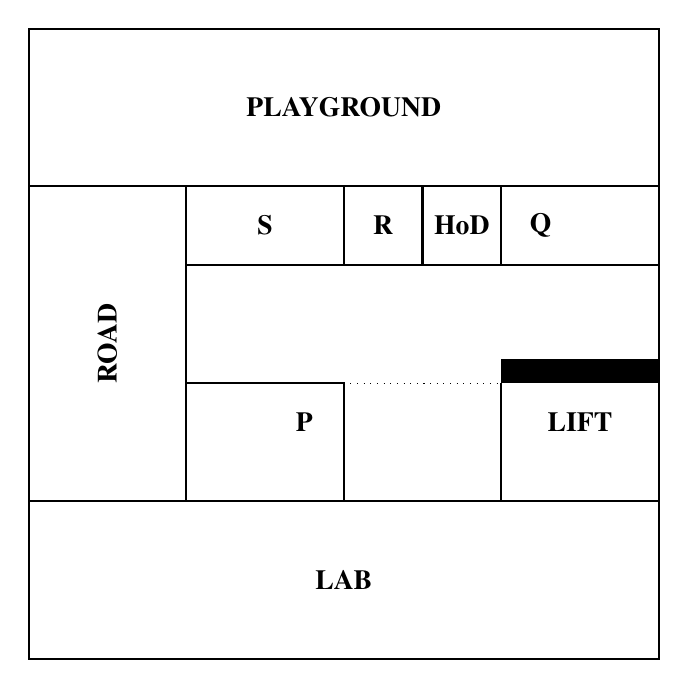
\begin{tikzpicture}
        % Outer boundary
        \draw[thick] (0,0) rectangle (8,8);
        
        % Divisions
        \draw[thick] (0,6) -- (8,6); % Horizontal line for playground
        \draw[thick] (0,2) -- (8,2); % Horizontal line for lab
        \draw[thick] (2,6) -- (2,2); % Vertical line for road
        \draw[thick] (6,3.5) -- (6,2); % Vertical line for lift
\draw[thick](2,5)--(8,5);
        % Playground and Lab Labels
        \node at (4,7) {\textbf{PLAYGROUND}};
        \node at (4,1) {\textbf{LAB}};

        % Road label
        \node[rotate=90] at (1,4) {\textbf{ROAD}};
        
        % Lift Label
        \node at (7,3) {\textbf{LIFT}};

        % HoD, Q, R, S labels
        \draw[thick] (2,6) -- (2,5); % Horizontal line for HoD row
        \draw[thick] (4,6) -- (4,5); % Vertical line for Q
        \draw[thick] (5,6) -- (5,5); % Vertical line for R
        \draw[thick] (6,6) -- (6,5); % Vertical line for S
        
        \node at (3,5.5) {\textbf{S}};
        \node at (4.5,5.5) {\textbf{R}};
        \node at (5.5,5.5) {\textbf{HoD}};
        \node at (6.5,5.5) {\textbf{Q}};

        % P label
        \draw[thick] (2,3.5) -- (4,3.5)--(4,2); % Horizontal line for P row
        \draw[dotted](4,3.5)--(6,3.5);
        \node at (3.5,3) {\textbf{P}};
        
        % Lift black bar
        \fill[black] (6,3.5) rectangle (8,3.8); % Thick black bar for the lift

    \end{tikzpicture}
  % Use the correct path to your Q4.tex file
    \end{figure}
       
        \item  \begin{figure}[H]
        \centering
        
    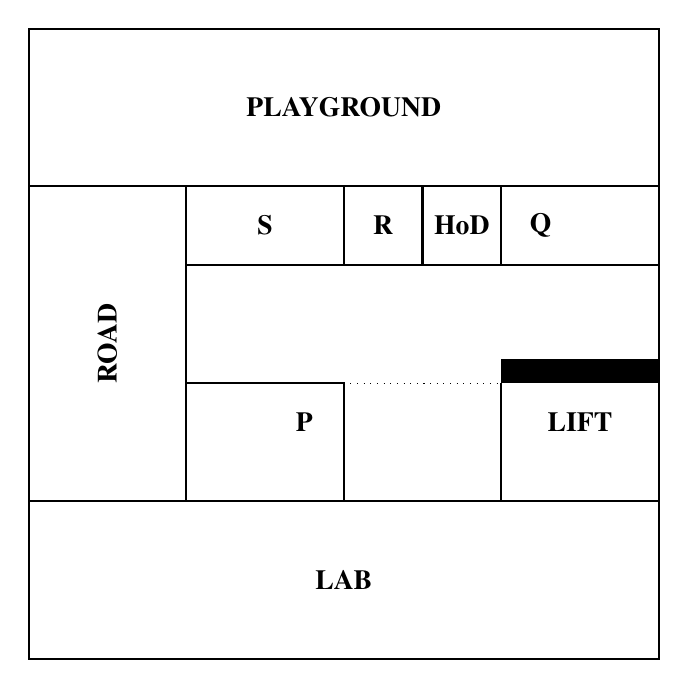
\begin{tikzpicture}
        % Outer boundary
        \draw[thick] (0,0) rectangle (8,8);
        
        % Divisions
        \draw[thick] (0,6) -- (8,6); % Horizontal line for playground
        \draw[thick] (0,2) -- (8,2); % Horizontal line for lab
        \draw[thick] (2,6) -- (2,2); % Vertical line for road
        \draw[thick] (6,3.5) -- (6,2); % Vertical line for lift
\draw[thick](2,5)--(8,5);
        % Playground and Lab Labels
        \node at (4,7) {\textbf{PLAYGROUND}};
        \node at (4,1) {\textbf{LAB}};

        % Road label
        \node[rotate=90] at (1,4) {\textbf{ROAD}};
        
        % Lift Label
        \node at (7,3) {\textbf{LIFT}};

        % HoD, Q, R, S labels
        \draw[thick] (2,6) -- (2,5); % Horizontal line for HoD row
        \draw[thick] (4,6) -- (4,5); % Vertical line for Q
        \draw[thick] (5,6) -- (5,5); % Vertical line for R
        \draw[thick] (6,6) -- (6,5); % Vertical line for S
        
        \node at (3,5.5) {\textbf{S}};
        \node at (4.5,5.5) {\textbf{R}};
        \node at (5.5,5.5) {\textbf{HoD}};
        \node at (6.5,5.5) {\textbf{Q}};

        % P label
        \draw[thick] (2,3.5) -- (4,3.5)--(4,2); % Horizontal line for P row
        \draw[dotted](4,3.5)--(6,3.5);
        \node at (3.5,3) {\textbf{P}};
        
        % Lift black bar
        \fill[black] (6,3.5) rectangle (8,3.8); % Thick black bar for the lift

    \end{tikzpicture}

  % Use the correct path to your Q4.tex file
    \end{figure}
       
        \item  \begin{figure}[H]
        \centering
        
    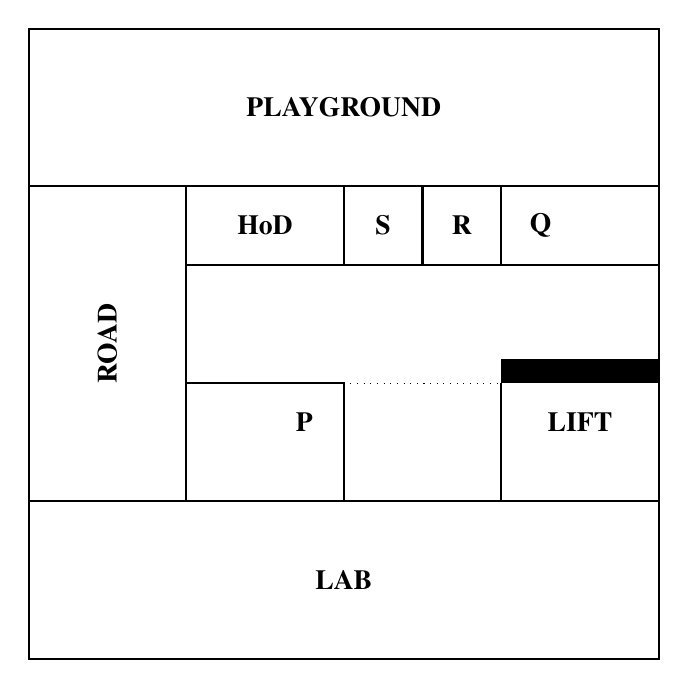
\begin{tikzpicture}
        % Outer boundary
        \draw[thick] (0,0) rectangle (8,8);
        
        % Divisions
        \draw[thick] (0,6) -- (8,6); % Horizontal line for playground
        \draw[thick] (0,2) -- (8,2); % Horizontal line for lab
        \draw[thick] (2,6) -- (2,2); % Vertical line for road
        \draw[thick] (6,3.5) -- (6,2); % Vertical line for lift
\draw[thick](2,5)--(8,5);
        % Playground and Lab Labels
        \node at (4,7) {\textbf{PLAYGROUND}};
        \node at (4,1) {\textbf{LAB}};

        % Road label
        \node[rotate=90] at (1,4) {\textbf{ROAD}};
        
        % Lift Label
        \node at (7,3) {\textbf{LIFT}};

        % HoD, Q, R, S labels
        \draw[thick] (2,6) -- (2,5); % Horizontal line for HoD row
        \draw[thick] (4,6) -- (4,5); % Vertical line for Q
        \draw[thick] (5,6) -- (5,5); % Vertical line for R
        \draw[thick] (6,6) -- (6,5); % Vertical line for S
        
        \node at (3,5.5) {\textbf{HoD}};
        \node at (4.5,5.5) {\textbf{S}};
        \node at (5.5,5.5) {\textbf{R}};
        \node at (6.5,5.5) {\textbf{Q}};

        % P label
        \draw[thick] (2,3.5) -- (4,3.5)--(4,2); % Horizontal line for P row
        \draw[dotted](4,3.5)--(6,3.5);
        \node at (3.5,3) {\textbf{P}};
        
        % Lift black bar
        \fill[black] (6,3.5) rectangle (8,3.8); % Thick black bar for the lift

    \end{tikzpicture}

  % Use the correct path to your Q4.tex file
    \end{figure}
       
    \end{enumerate}

    \item The number of students in three classes is in the ratio 3:13:6. If 18 students are added to each class, the ratio changes to 15:35:21.
    
    The total number of students in all the three classes in the beginning was:
    \begin{enumerate}
        \item 22
        \item 66
        \item 88
        \item 110
    \end{enumerate}

    \item The number of units of a product sold in three different years and the respective net profits are presented in the figure below. The cost/unit in Year 3 was 1, which was half the cost/unit in Year 2. The cost/unit in Year 3 was one-third of the cost per unit in Year 1. Taxes were paid on the selling price at 10\%, 13\%, and 15\% respectively for the three years. Net profit is calculated as the difference between the selling price and the sum of cost and taxes paid in that year.
    
   \begin{figure}[H]
        \centering
        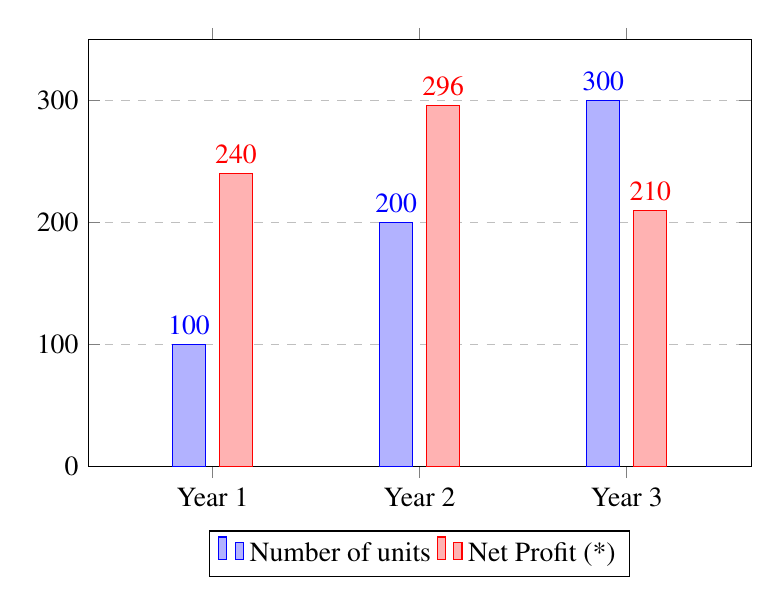
\begin{tikzpicture}
\begin{axis}[
    ybar=5pt,
    bar width=12pt,
    width=10cm, height=7cm,
    ymin=0, ymax=350,
    ylabel={},
    symbolic x coords={Year 1, Year 2, Year 3},
    xtick=data,
    nodes near coords,
    legend style={at={(0.5,-0.15)},anchor=north,legend columns=-1},
    enlarge x limits=0.3,
    ymajorgrids=true,
    grid style=dashed
]

\addplot coordinates {(Year 1, 100) (Year 2, 200) (Year 3, 300)};
\addplot coordinates {(Year 1, 240) (Year 2, 296) (Year 3, 210)};

\legend{Number of units, Net Profit (*)}

\end{axis}
\end{tikzpicture}  % Use the correct path to your Q4.tex file
    \end{figure}
       
    
    The ratio of the selling price in Year 2 to the selling price in Year 3 is:
    \begin{enumerate}
        \item $4:3$
        \item $1:1$
        \item $3:4$
        \item $1:2$
    \end{enumerate}

    \item Six students P, Q, R, S, T, and U, with distinct heights, compare their heights and make the following observations:
    
    Observation I: S is taller than R. \\
    Observation II: Q is the shortest of all. \\
    Observation III: U is taller than only one student. \\
    Observation IV: T is taller than S but is not the tallest.
    
    The number of students that are taller than R is the same as the number of students shorter than {\underline{\hspace{2cm}}}.
    \begin{enumerate}
        \item T
        \item R
        \item S
        \item P
    \end{enumerate}
\end{enumerate}
\section*{Engineering Mathematics (XE-A)}

\subsection*{Q.1 - Q.3 Multiple Choice Questions (MCQs),carry \textbf{ONE} mark each (For each wrong answer: $-\frac{1}{3}$).
}

\begin{enumerate}
    \item Let 
    $$s = \brak{A x : A = \begin{bmatrix} 2 & -4 \\ 1 & 1 \\ 1 & -1 \end{bmatrix} and X = \begin{bmatrix} x_1 \\ x_2 \end{bmatrix}}.$$
    If $\begin{bmatrix}
        -1\\\alpha\\1
    \end{bmatrix} \in S$, then the value of $\alpha$ is
    \begin{enumerate}
        \item $-4$
        \item $-2$
        \item $2$
        \item $4$
    \end{enumerate}

    \item Let $C$ be the boundary of the region $R: 0 < x < \pi, 0 < y < \sin x$ in the $xy$-plane, and $A$ be the area of the region $R$. If $C$ is traversed once in the counterclockwise direction, then the value of the line integral $\oint_C (2y \, dx + 5x \, dy)$ is:
    \begin{enumerate}
        \item $\alpha$
        \item $2\alpha$
        \item $3\alpha$
        \item $4\alpha$
    \end{enumerate}

    \item Given that $i = \sqrt{-1}$, the value of 
    $$\lim_{z \to e^\frac{{\pi}i}{3}} \frac{z^3 + 1}{z^4+z^2 + 1}$$ is
    \begin{enumerate}
        \item $\frac{3}{4} + i \frac{\sqrt{3}}{4}$
        \item $\frac{3}{4} - i \frac{\sqrt{3}}{4}$
        \item $-\frac{3}{4} + i \frac{\sqrt{3}}{4}$
        \item $-\frac{3}{4} - i \frac{\sqrt{3}}{4}$

    \end{enumerate}
\end{enumerate}

\end{document}